\documentclass[xcolor={dvipsnames}]{beamer}
\mode<presentation>{\usetheme{boxes}}
\usecolortheme{default}
\setbeamertemplate{navigation symbols}{}%remove navigation symbols

\setbeamerfont{frametitle}{size=\Large}

%\setbeamercolor{structure}{fg=beamer@blendedblue}



\setbeamertemplate{bibliography item}{\insertbiblabel}

\setbeamercolor{bibliography entry author}{fg=black}
\setbeamercolor{bibliography entry title}{fg=black} 
\setbeamercolor{bibliography entry location}{fg=black} 
\setbeamercolor{bibliography entry note}{fg=black}  

\usepackage[style=numeric,sorting=ydnt,maxnames=1,defernumbers=true, firstinits=true]{biblatex}
\renewbibmacro{in:}{}
\ExecuteBibliographyOptions{sorting=ydnt}

%\addbibresource{./jlescSummerSchool_checkpointing.bib}

\makeatother
\setbeamertemplate{footline}
{
  \leavevmode%
  \hbox{%
    %% \begin{beamercolorbox}[wd=.2\paperwidth,ht=2.25ex,dp=1ex]{date in head/foot}%
    %%   \usebeamerfont{date in foot}
    %% \end{beamercolorbox}%
  %%   \begin{beamercolorbox}[wd=.6\paperwidth,ht=2.25ex,dp=1ex, center]{date in head/foot}%
  %%     \usebeamerfont{date in foot}\insertshortdate
  %% \end{beamercolorbox}%
  \begin{beamercolorbox}[wd=\paperwidth,ht=2.25ex,dp=1ex]{date in head/foot}%
    \usebeamerfont{date in foot}\hfill
    {\scriptsize\insertframenumber{}}\hspace*{2ex}
  \end{beamercolorbox}}%
  \vskip0pt%
}
\makeatletter



\usepackage[utf8]{inputenc}
%\usepackage[T1]{fontenc}
%\usepackage[francais]{babel}
\usepackage{hyperref}
\usepackage{url}
\usepackage{pifont}
\usepackage{changepage}
\usepackage{listings}
\lstset{basicstyle=\ttfamily,
  showstringspaces=false,
  commentstyle=\color{black},
  keywordstyle=\color{black}
}

\usepackage{fancyvrb}
\usepackage{multirow}
\usepackage{tabu} 
\usepackage{colortbl}

\usepackage{marvosym}

\usepackage{eurosym}

%\usepackage{gitdags}
\usepackage{comment}

\usepackage{pdfpages}
\setbeamercolor{background canvas}{bg=}


\usepackage{perpage} %the perpage package
\MakePerPage{footnote}



\definecolor{beamer@blendedblue}{RGB}{0,102,204}

\definecolor{beamer@lightgray}{RGB}{238,238,224}


\definecolor{itemorange}{RGB}{255,114,0}


\definecolor{myorange}{RGB}{255,103,0}


\setbeamertemplate{itemize items}[circle]
\setbeamertemplate{itemize subitem}[triangle]


\setbeamercolor{itemize item}{fg=beamer@blendedblue}
\setbeamercolor{itemize subitem}{fg=gray}


\newcommand<>{\Blue}[1]{{\color#2{beamer@blendedblue}#1}}
%\newcommand<>{\Orange}[1]{{\color#2{BurntOrange}#1}}
\newcommand<>{\Orange}[1]{{\color#2{myorange}#1}}
\newcommand<>{\Alert}[1]{{\Orange{\textbf{#1}}}}


\newcommand{\largeskip}{\vspace{0.6cm}}
\newcommand{\hugeskip}{\vspace{1cm}}



\usepackage{tikz}
\usetikzlibrary{%
decorations.pathreplacing,%
decorations.pathmorphing,%
decorations.shapes,%
decorations.text,%
decorations.markings,%
shapes,%
shapes.callouts,%
shadows,%
arrows,
calc,%
positioning,%
chains,%
backgrounds,%
fit, %
fadings}

\tikzset{
    invisible/.style={opacity=0},
    visible on/.style={alt={#1{}{invisible}}},
    alt/.code args={<#1>#2#3}{%
      \alt<#1>{\pgfkeysalso{#2}}{\pgfkeysalso{#3}} % \pgfkeysalso doesn't change the path
    },
}


\tikzset{
    colornode/.style={
        outer sep=0pt, fill=#1!67, %text height=2ex, text depth=.5ex
    },
    cpu/.style={
        diamond, fill=gray!30, aspect=3, name=CPU#1,
        node contents={$\text{CPU}_{#1}$},
    },
    thread/.style={fill=#1!67,
        minimum width=5ex, minimum height=1.25em},
    tick/.style={very thin},
}



\newcommand{\email}[1]{\href{mailto:#1}{\nolinkurl{#1}}}

\newcommand{\xmark}{\ding{55}}


\AtBeginPart{
  %\frame{\partpage}
  \frame{
    \frametitle{Agenda}
    \small
    \tableofcontents[part=\insertpartnumber,
    sectionstyle=show,
    subsectionstyle=hide,
    subsubsectionstyle=hide]
  }
}

\AtBeginSection[]
{
  \begin{frame}
    \frametitle{Agenda}
    \small
    \tableofcontents[
    sectionstyle=show/shaded,
    subsectionstyle=show/show/hide,
    subsubsectionstyle=hide]
  \end{frame}
}

\AtBeginSubsection[]{
  \mode<presentation>{
    \frame{\tableofcontents[
      sectionstyle=show/hide,
      subsectionstyle=show/shaded/hide,
      subsubsectionstyle=show/show/hide]
    }
  }
}


\date[\the\year]{\the\year}

\newcommand{\shellcmd}[1]{\indent\indent\texttt{\footnotesize\$ #1}}


\title[]{Cloud Computing}
\subtitle{Concepts de virtualisation\footnote{Adapté du support développé par Thomas ROPARS et Renaud LACHAIZE}}

%Thomas ROPARS : \url{https://tropars.github.io/teaching/},
%\url{https://roparst.gricad-pages.univ-grenoble-alpes.fr/cloud-tutorials/m2gi-devops/}}}


\author[]{\\Danilo Carastan dos Santos
  \\ \vspace{0.5cm} \email{danilo.carastan-dos-santos@univ-grenoble-alpes.fr}}

\definecolor{mybrown}{RGB}{205,133,63}
\definecolor{myblue}{RGB}{28,134,238}

\let\Red=\alert
\newcommand<>{\green}[1]{{\color#2{green!70!black}#1}}
\newcommand<>{\blue}[1]{{\color#2{blue!100!black!100}#1}}
\definecolor{darkgreen}{rgb}{0,0.5,0}

\newcommand\myvdots{{\smash[b]\strut\smash[t]\vdots}}


\usepackage{boxedminipage}
\newenvironment{boitecode}[1]{
    \begin{boxedminipage}{\linewidth}      
%\begin{beamerboxesrounded}[shadow=true,lower=lightex,upper=medex]{#1}
    #1
    \begin{semiverbatim}
}{   \end{semiverbatim}\vspace{-1.5\baselineskip}
    \end{boxedminipage}
%  \end{beamerboxesrounded}
}


\begin{document}


\begingroup
\setbeamercolor{titlelike}{bg=beamer@lightgray, fg=black}
\begin{frame}
\titlepage
\end{frame}
\endgroup

\begin{frame}{Problematique}
    \begin{columns}
        \begin{column}{.4\linewidth}
            
                Applications : 
                \begin{itemize}
                    \item Email
                    \item Partage de données
                \end{itemize}
                Chaque application a de prérequis spécifiques de ressources physiques/logiciels
                \begin{itemize}
                    \item Utilisation de CPU
                    \item Mémoire
                    \item Stockage
                    \item Système d'exploitation
                    \item Librairies/Intergiciels spécifiques
                \end{itemize}            
        \end{column}
        \begin{column}{.6\linewidth}            
            \centering 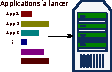
\includegraphics[width=\linewidth]{Figures/data-center-virt-1.pdf}
        \end{column}
    \end{columns}    
\end{frame}

\begin{frame}{Une première solution naïve}
    \begin{columns}
        \begin{column}{.4\linewidth}
            \begin{itemize}
                \item Une application par serveur
                \item Inconvénient : sous-utilisation des serveurs
            \end{itemize}
        \end{column}
        \begin{column}{.6\linewidth}            
            \centering 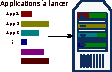
\includegraphics[width=\linewidth]{Figures/data-center-virt-2.pdf}
        \end{column}
    \end{columns}    
\end{frame}

\begin{frame}{Une deuxième solution}
    \begin{columns}
        \begin{column}{.4\linewidth}
            \begin{itemize}
                \item Plusieurs applications par serveur
                \item Problèmes : 
                \begin{itemize}
                    \item Contrôle de ressources
                    \item Isolation d'applications                     
                \end{itemize}
            \end{itemize}
        \end{column}
        \begin{column}{.6\linewidth}            
            \centering 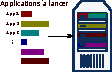
\includegraphics[width=\linewidth]{Figures/data-center-virt-3.pdf}
        \end{column}
    \end{columns}   
    Exemple : 
    \begin{itemize}
        \item  Apps A et B tournent dans un même serveur. App A a besoin une
        mise à jour du système d'exploitation. Cette MàJ peut affecter B. 
    \end{itemize} 
\end{frame}

\begin{frame}{Une meilleure solution : virtualisation}

    \begin{itemize}
        \item \textbf{Idée :} Créer plusieurs ressources virtuelles (Machine Virtuelle - VM) à partir
        d'une ou plusieurs ressources physiques        
        \item Dans une VM nous ne pouvons pas distinguer entre ressources
        physiques ou virtuelles
        \item \textbf{Concept clé :} Hyperviseur
        \begin{itemize}
            \item Est une couche logicielle
            \item Fournit l’abstraction d’une ou plusieurs machines ``nues''
            (processeurs, mémoire et périphériques) au-dessus d’une véritable
            machine physique
        \end{itemize}
        \item Intérêt : 
        \begin{itemize}
            \item Faire tourner plusieurs systèmes d’exploitation simultanément
            sur la même plateforme matérielle
            \item Sauvegarder/rembobiner l’état d’un système
            \item Sécurité (renforcement de l’isolation de certaines
            applications)
        \end{itemize}
    \end{itemize} 
\end{frame}

\begin{frame}{Virtualisation}
\begin{itemize}
    \item Hyperviseur de type I (natif) : Couche logicielle de plus bas
    niveau. Système d’exploitation spécialisé. Plus efficace    
    \item Exemples : VMware ESX, Xen
    \item Hyperviseur de type II (hébergé) : Application intermédiaire (intergiciel) qui s’appuie sur un système hôte sous-jacent
    \item Moins efficace (plus de couches) mais plus simple à installer/utiliser
    \item Exemples : VMware workstation/fusion/player, VirtualBox
\end{itemize}

    \centering 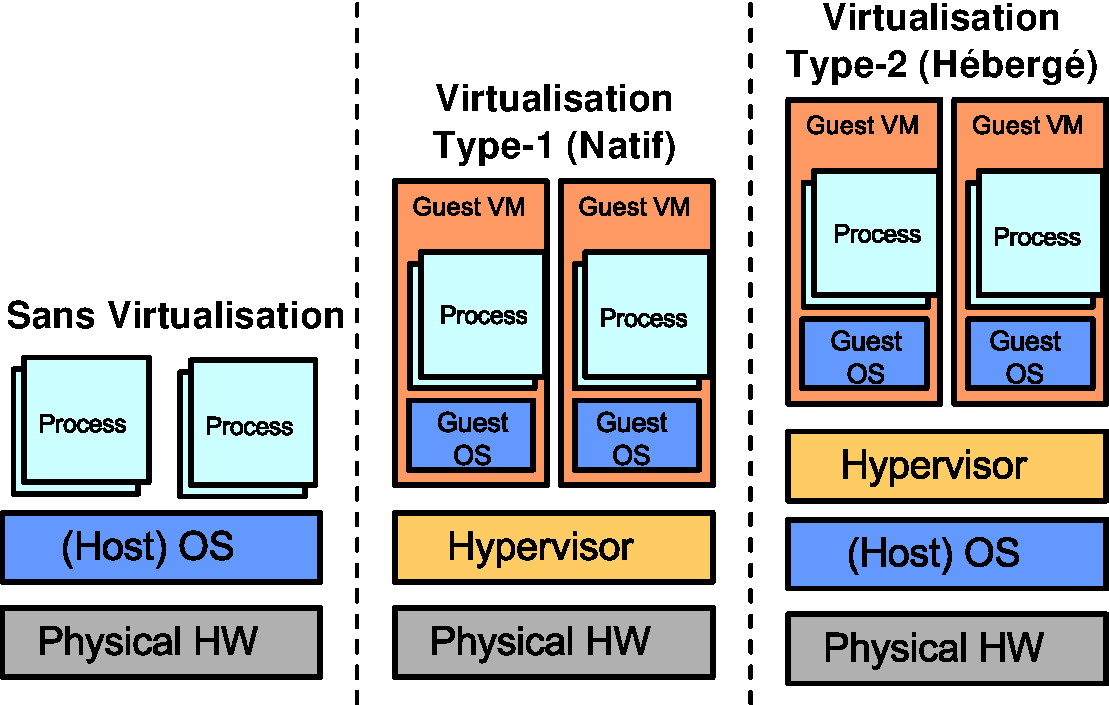
\includegraphics[width=.7\linewidth]{Figures/virtualisation.pdf}
\end{frame}


\begin{frame}{Image d'une machine virtuelle}
    \begin{itemize}
        \item Snapshot of a virtual machine
        \item Allows for a faster deployment of VMs. No need to install OS +
        additional software every time a vm is launched
    \end{itemize}
    
\end{frame}

\begin{frame}{Scalabilité}{\textit{Scaling}}
    \begin{itemize}
        \item Terme générique lié au comportement d'une application si la charge
        de travail et/ou les ressources changent
        \item Deux types : 
        \begin{itemize}
            \item \textbf{Scalabilité faible (Weak scaling) :} ``Puis-je faire plus de travail (traiter
            plus de requêtes, traiter plus de données) si j'ai plus de
            ressources ?''  
            \item \textbf{Scalabilité forte (Strong scaling) : } ``Puis-je faire la même charge
            de travail dans moins de temps si j'ai plus de ressources ?''
        \end{itemize}
    \end{itemize}
\end{frame}

\begin{frame}{Elasticité}{\textit{Autoscaling}}
    \begin{itemize}
        \item \textbf{Idée générale : } Adapter les ressources en fonction de la charge de travail courante
        \item Exemple : ``Mon application de commerce électronique basée sur le
        Web devrait traiter n'importe quelle requête en moins de 500 ms, quel
        que soit le nombre total de requêtes qu'elle traite actuellement.''
        \item ``Juste ce qu'il faut'' :
        \begin{itemize}
            \item Pas assez de ressources $\rightarrow$ traitement plus long
            (perte de qualité de service)
            \item Trop de ressources $\rightarrow$ ressources non utilisées (et
            on les paye quand même)
        \end{itemize}
        %\item Pour certains services Cloud, l'Élasticité est transparente pour les utilisateurs
    \end{itemize}
\end{frame}

\begin{frame}{Scalabilité Verticale}{\textit{Vertical Scaling}}

    \begin{columns}
        \begin{column}{.4\linewidth}
            \begin{itemize}
                \item \textbf{Idée : } remplacer les machines (virtuelles) avec des
                machines (virtuelles) plus puissantes
                \item \textbf{Avantages : }
                \begin{itemize}
                    \item Plus simple                    
                \end{itemize}
                \item \textbf{Inconvénients : }
                \begin{itemize}
                    \item Scalabilité limitée 
                    \item Coût non linéaire de ressources                    
                \end{itemize}
            \end{itemize}        
        \end{column}
        \begin{column}{.6\linewidth}            
            \centering 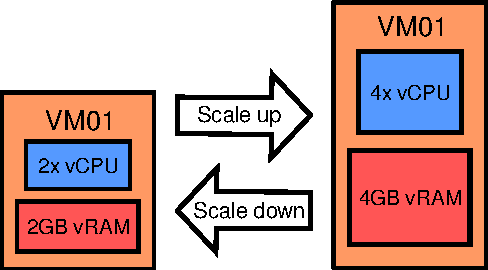
\includegraphics[width=.9\linewidth]{Figures/virtual-scaling.pdf}
        \end{column}
    \end{columns}   

   
    
    
\end{frame}

\end{document}